\documentclass{article}
\usepackage[utf8]{inputenc}
\usepackage[legalpaper, portrait, margin=1in]{geometry}
\usepackage{enumitem}
\usepackage{graphicx}


\title{CS 156a Set 2}
\author{Cason Shepard}
\date\today

\begin{document}

\maketitle
{\Large The following algorithm was used to answer questions 1-2}
\begin{verbatim}
import random
import numpy

def coinflip():
    return int(numpy.floor(random.randint(0,1)))


v_1 = 0
v_rand = 0
v_min = 0

for x in range(0, 100000):
    if x%1000 == 0:
    freq_1000 = [0] * 1000
    for i in range(0, 1000):
        coin_10 = [0] * 10
        for q in range(0,10):
            coin_10[q] = coinflip()
        heads_frequency = sum(coin_10)/10
        freq_1000[i] = heads_frequency
    v_1 = v_1 + freq_1000[0]/100000
    v_rand = v_rand + random.choice(freq_1000)/100000
    v_min = v_min + min(freq_1000)/100000

print(v_1)
print(v_rand)
print(v_min)
\end{verbatim}

\section*{problem 1}
After running the algorithm above, the average value for $v_min$ over 100000 iterations was 0.037869. This is closest to 0.01.\\
\newline
\textbf{The answer is [b]}

\section*{problem 2}
After running the algorithm above, the average values for $v_1$, $v_{rand}$, and $v_{min}$ were:
\begin{center}
$v_1 = 0.4998539999997137$\\
$v_{rand} = 0.5009359999997081$\\
$v_{min} = 0.03786900000001721$    
\end{center}
In order for a distribution of $v$ to satisfy the Hoeffding (single-bin) Inequality, $v$ must be close to the true probability of flipping a coin and getting heads. Thus, the only two values that satisfy this are $v_1$ and $v_{rand}$.
\newline\newline
\textbf{The answer is [d]}

\section*{problem 3}
Since we are interested in the probability of error that $h$ makes in approximating $y$ given the noisy data, we must consider the event in which we either get a false-positive or false-negative result by the confusion matrix below. By adding the error boxes, we get the probability of error: $(1-\lambda) * (1-\mu) + \lambda * \mu$
\fbox{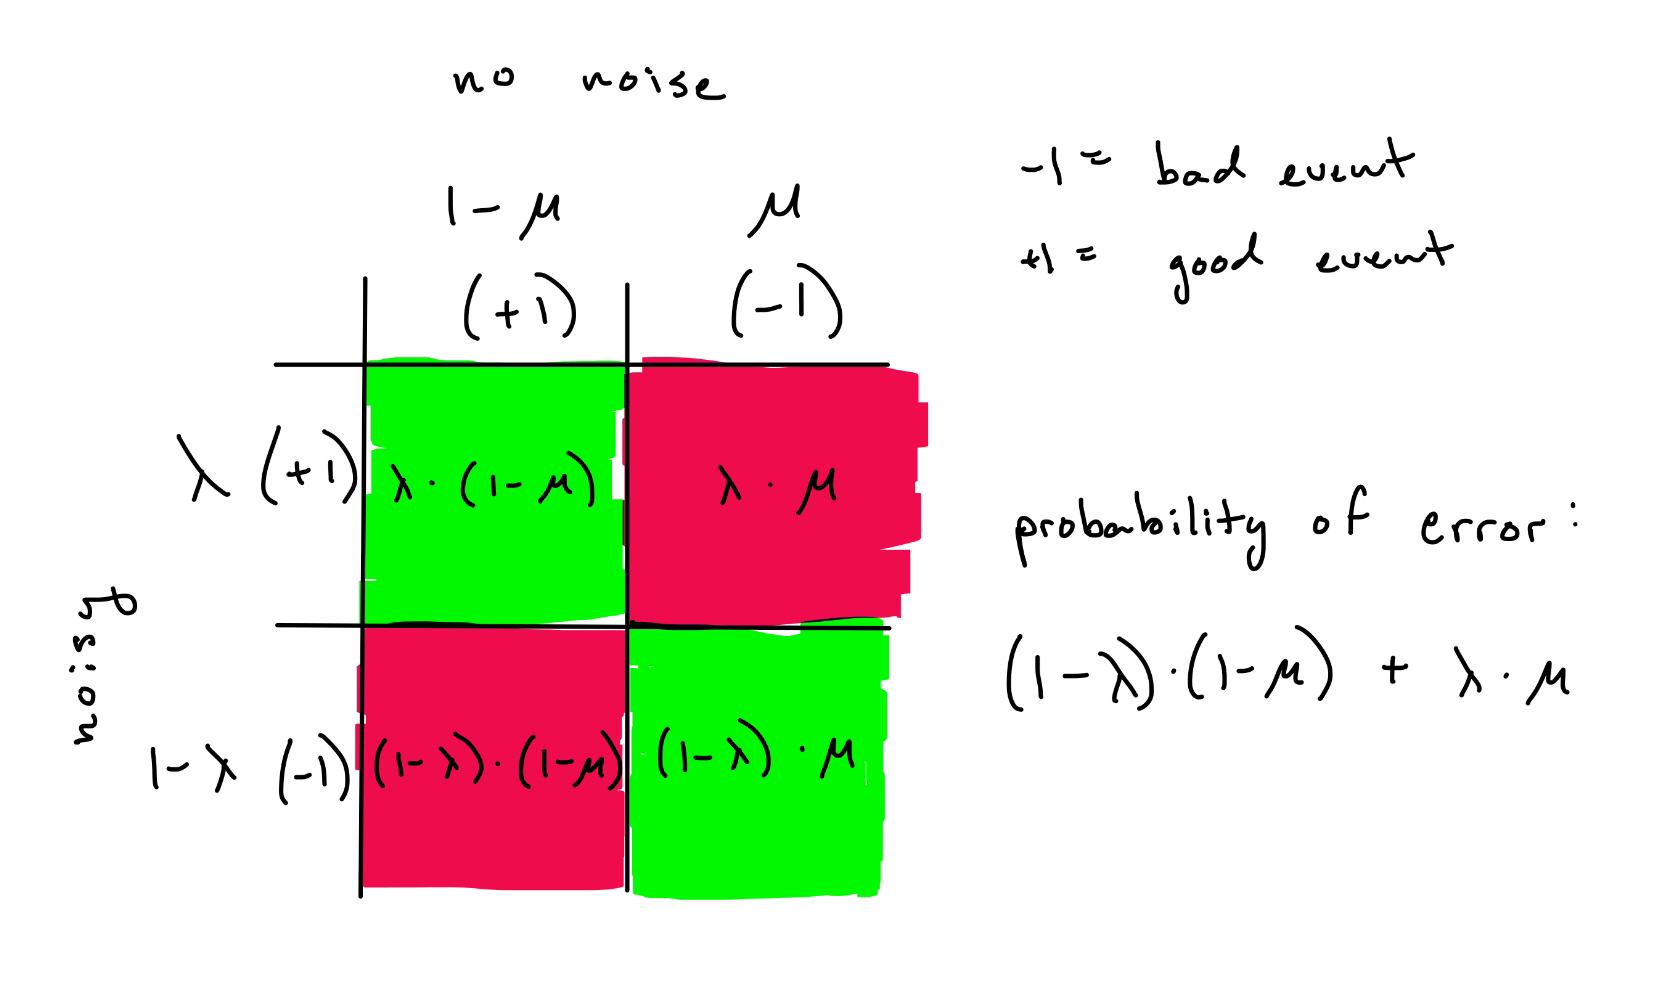
\includegraphics[width=\textwidth]{confusion_matrix.png}}\\ \\
\textbf{The answer is [e]}

\section*{problem 4}
To find when $h$ is independent of $\mu$, we must find the value of $\lambda$ where $\mu$ can be eliminated from the equation:
\begin{center}
    $\epsilon = (1-\lambda) * (1-\mu) + \lambda * \mu$\\
    $\epsilon = 1  - \mu - \lambda + \lambda\mu + \lambda\mu$\\
    $\epsilon = 1 - \mu * (2\lambda - 1)$\\
    To eliminate $\mu$, we can set $2\lambda - 1$ equal to 0 and solve for $\lambda$. This gives us:\\
    $\lambda = 0.5$
\end{center}
\textbf{The answer is [b]}
\newpage
{\Large The following Linear Regression algorithm was used/manipulated to answer questions 5-10. The algorithm was made into one function so that it could be iterated 1000 times with ease later.}
\begin{verbatim}

from random import uniform
import numpy
import random

def Lin_Reg():
    #SETUP
    """x_1 = uniform(-1, 1)
    y_1 = uniform(-1, 1)
    x_2 = uniform(-1, 1)
    y_2 = uniform(-1, 1)

    a, b = numpy.polyfit([x_1, y_1], [x_2, y_2], 1)"""

    def f(x, y): #target function
        return (x*x + y*y - .6)

    def sign(x):
        if x == 0:
            return 0
        elif x > 0:
            return 1
        else:
            return -1
    
    def count_diff(list_1, list_2):
        count = 0
        for x in range(0, len(list_1)):
            if list_1[x] != list_2[x]:
                count += 1
        return count
    
    N = 1000
    y_target = [0] * N
    point_list = [] * N
    classification_list = [0] * N
    PLA = [0] * N
    
    for i in range(0,N):
        temp_x1 = uniform(-1, 1)
        temp_x2 = uniform(-1, 1)
        point_list.append([1, temp_x1, temp_x2, temp_x1*temp_x2, temp_x1*temp_x1, temp_x2*temp_x2])
        y_target[i] = f(point_list[i][1], point_list[i][2])

    y_data = [x[2] for x in point_list] 

    for i in range(0,N):
        if sign(y_target[i]) == 1:
            classification_list[i] = 1
        else:
            classification_list[i] = -1
    
    idx_array = random.sample(range(0, 1000), 100)
    for x in range(0, 100):
        classification_list[int(idx_array[x])] = classification_list[int(idx_array[x])] * -1
    
    idx_array = 1000 * numpy.random.sample((100,))
    X_points = numpy.array(point_list)
    X_dagger = numpy.matmul(numpy.linalg.pinv(numpy.matmul(X_points.T, X_points)), X_points.T)
    w = numpy.matmul(X_dagger, numpy.array(classification_list))

    E_in = (1/N)*numpy.dot(numpy.subtract(numpy.matmul(X_points, w), classification_list),numpy.subtract(numpy.matmul(X_points, w), classification_list))
    
    """
    itter_count = 0
    while PLA != classification_list:
        itter_count = itter_count + 1
        wrong = []
        for p in range(0, N):
            if classification_list[p] != PLA[p]:
                wrong.append(p)
        index_point = random.choice(wrong)
        random_point_x = point_list[index_point]        
        #grab sign of correct classification
        temp_sign = classification_list[index_point]
        # unpack and repack weight tuple
        w = [w[0] + temp_sign*random_point_x[0], w[1] + temp_sign*random_point_x[1], w[2] + temp_sign*random_point_x[2]]
        PLA = [0] *N
        for idx in range(0, len(PLA)):
            if numpy.dot(point_list[idx], w) > 0:
                PLA[idx] = 1
            else:
                PLA[idx] = -1
                """
    
    y_correct = [0] * 1000
    points = []
    classification = [0] * 1000
    classification_check = [0]*1000

    for i in range(0,1000):
            temp_x1 = uniform(-1, 1)
            temp_x2 = uniform(-1, 1)
            points.append([1, temp_x1, temp_x2, temp_x1*temp_x2, temp_x1*temp_x1, temp_x2*temp_x2])
            y_correct[i] = f(points[i][1], points[i][2])
    
    y_random = [x[2] for x in points] 

    for i in range(0,1000):
        if sign(y_correct[i]) == 1:
            classification[i] = 1
        else:
            classification[i] = -1
    
    idx_array = random.sample(range(0, 1000), 100)
    for x in range(0, 100):
        classification[int(idx_array[x])] = classification[int(idx_array[x])] * -1

    for idx in range(0, len(classification_check)):
        if numpy.dot(points[idx], w) > 0:
            classification_check[idx] = 1
        else:
            classification_check[idx] = -1
                
    diff = count_diff(classification, classification_check)
    E_out = diff/1000

            
    return (E_out, E_in, w)
\end{verbatim}

\section*{problem 5}
After 1000 iterations, my algorithm got an $E_{in}$ of 0.0389, which is closest to 0.01.\\\\
\textbf{The answer is [c]}

\section*{problem 6}
After 1000 iterations, my algorithm got an $E_{out}$ of 0.04852, which is closest to 0.01.\\\\
\textbf{The answer is [c]}

\section*{problem 7}
After processing the PLA using the $w$ value determined by the linear regression algorithm, the PLA converged in an average of 5.9 iterations over 1000 trials. This is closest to 1.\\\\
\textbf{The answer is [a]}

\section*{problem 8} 
After carrying out the linear regression on the new target function with the added noise, I got an average value of 0.6974350480139204 for $E_{in}$ over 1000 trials. This is closest to 0.8.\\\\
\textbf{The answer is [e]}

\section*{problem 9}
After transforming the $w$ vector to $\tilde{w}$ and running this algorithm 1000 times, the average $\tilde{w}$ values were:
\begin{center}
    $\tilde{w} = (-.9916, -.0009, -.0002, .0054, 1.560, 1.557)$
\end{center}
These values are closest to the coefficients of the function of [a].\\\\
\textbf{The answer is [a]}

\section*{problem 10}
After running this algorithm on a new set of data outside the original sample, including noise, the average $E_{out}$ over 1000 trials was 0.126 which is closest to 0.1.\\\\
\textbf{The answer is [b]}

\end{document}
